\chapter{序論}
\label{chap::intro}

\section{研究背景}
オフィスビルなどの建物を含む業務部門のCO$_2$排出量は,日本全体のCO$_2$排出量のうち約2割を占めており,他部門に対して増加量が多い\cite{EDMC15}.そのため,オフィスビルにおけるエネルギー消費量およびCO$_2$排出量の削減が喫緊の課題となっている.そこで,ビルの新築・改修時に設計段階において,年間のエネルギー消費量を一定以下にするnZEB (net Zero Energy Building)化の動きが広まっている\cite{Shigen16}.また,ビルの運用段階においてもエネルギー消費量を削減する取り組みがある.一般的なオフィスビルでは,総エネルギー消費量のうち,空調設備による消費が約3割を占める\cite{Kanto11}.空調システムによるエネルギー消費量は,設定温度や気象条件,オフィスルームの使用状況などの要因によって変動する.これらの要因に合わせた空調設備の運用改善によるエネルギー消費量の削減が期待されている\cite{EIA17, Enecho17}.一方,オフィスビルでは,室内環境の改善によるオフィスワーカーの快適性維持向上も必要である.これまでの空調設備の運用によるエネルギー消費量の削減手段は,しばしば室内環境の悪化とオフィスワーカーの快適性の低下を伴うものだったが,このような環境はオフィスワーカーの知的生産性を低下させる\cite{Iwahashi14}.また,室内快適性の向上は,オフィスワーカーの健康増進に寄与するほか,離職率の低下など投資に値する効果があることが報告されている\cite{WGBC14}.そのため,オフィスの快適性を維持しながらエネルギー消費量を削減できる空調設備の運用方法が求められる.

空調設備運用によるエネルギー消費量削減の目標達成の考え方として,オフライン制御とオンライン制御の2つがどちらも必要である\cite{Kamimura08}.オンライン制御とオフライン制御の関係を\figref{fig::intro_offline}に示す.オフライン制御は,エネルギー消費量の目標値から求めた当日使用可能なエネルギー消費量および気象予報などの情報から事前に空調設定の計画値を決定し,計画値に合わせて空調設定を変更する.一方でオンライン制御は,実際のエネルギー消費量や室内の快適度,外気温などから,リアルタイムに空調設定値をより効果的なものに変更する.nZEBで求められる1年といったスパンでエネルギー消費量を管理するためには,日毎の計画値をオフライン制御で定めてオンライン制御の目標値とすることが重要であることから,本論文では,オフィスビルの空調設備の運用のオフライン制御に着目する.

% オフライン制御とオンライン制御の図
\begin{figure}[ht]
    \begin{center}
        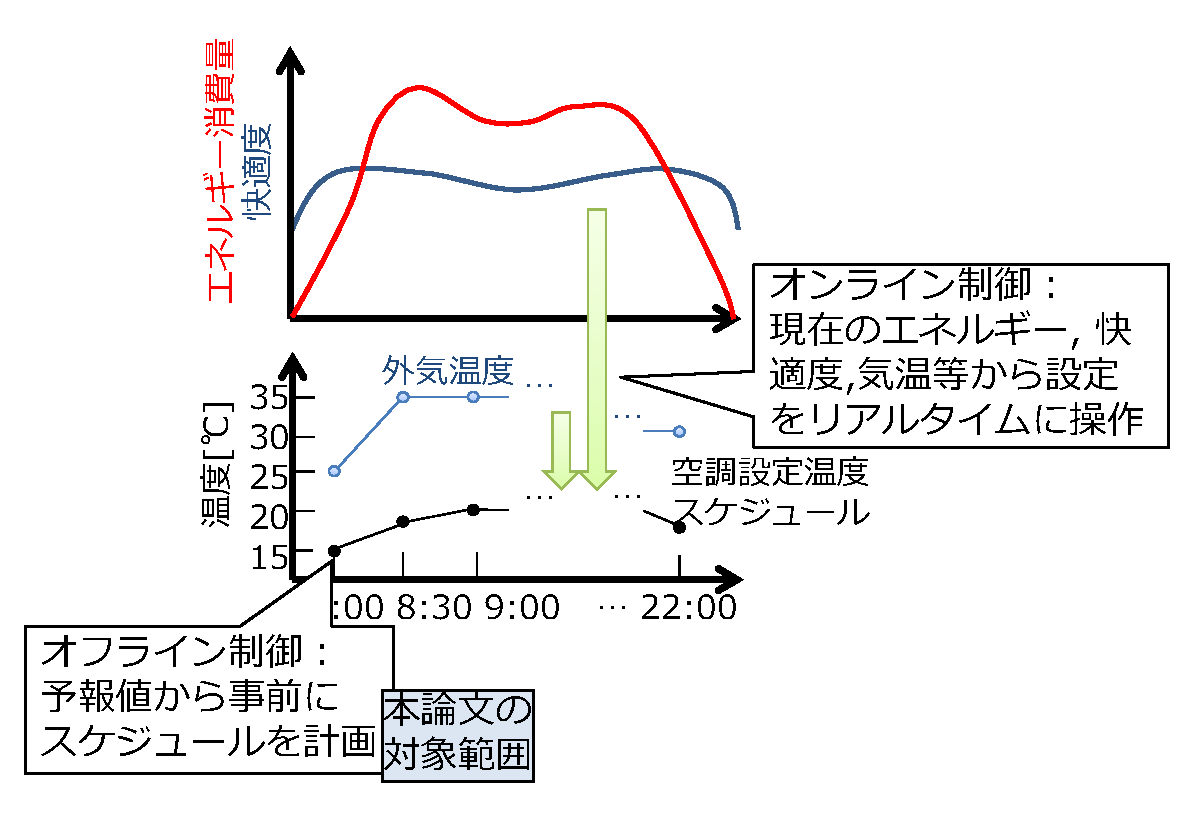
\includegraphics[width=0.6\textwidth,keepaspectratio=true]{fig/intro_offline.eps}
    \end{center}
    \caption{空調設定のオフライン制御とオンライン制御の関係}
    \label{fig::intro_offline}
\end{figure}

通常,ビルの空調設定は,ビル管理者により過去のエネルギー消費量データに基づいて季節や月・日単位で設定される.気象条件が通常と異なる場合やエネルギー消費量が目標値を超える恐れがある場合には,ビル管理者が空調設定を変更する.しかしながら,この運用はビル管理者のKKD(勘・経験・度胸)に頼ったものであることが多く,十分な節電ができない場合や,過度に節電してしまいオフィスの快適性の低下を招くことがある.また,十分な経験がない管理者には判断が難しい.そこで,空調設備の運用改善とビル管理者の業務省力化のために,空調設定計画の詳細なスケジュールを適切に決定する手法が必要である.

これまでに,空調設定計画の事前スケジューリングに対して,最適化手法を用いる方法が研究されている.単一目的の最適化手法を用いる方法として,1つは,室内の環境を快適に保つことができる空調機の設定の組合せのうちエネルギー消費量が最小になる組合せを探す,といったように快適性とエネルギー消費量のうちどちらか一方を制約条件とし,もう一方を目的関数に設定する方法がある\cite{Alhaider15, Ueda10, Xu13}.また,快適性とエネルギー消費量の重み付け和を目的関数として,1つの目的関数を持つ数理計画問題として解く方法がある\cite{Takagi11, Xiao17}.しかし,これらの単一目的の最適化手法では,重みや制約によってどの程度快適性もしくはエネルギー消費量が変化するかを事前に知ることができず,重みや制約値の決定が難しい.さらに,最適化によって得られる単一の最適解をそのまま適用するほかなく,例えば当日使用可能なエネルギー量に余力があり快適性を優先した設定としたい場合や,エネルギー量に制限が発生した場合などにスケジュールを調整することが困難である.そこで,エネルギー消費量と快適性を同時に追究する空調運用のため,多目的最適化による空調設定スケジュールの最適化手法が提案されてきた.

空調設定スケジューリングへの多目的最適化の適用事例として,エネルギー消費量ピークの抑制による電気料金の削減と快適な温度設定の維持を目的関数として適用した事例がある\cite{Zhang14}.この事例では,電気料金および室内温度をそれぞれ独立した目的関数として取り扱い,2つの目的の間のパレート解を探索している.一方で,目的関数はエネルギーや快適性を直接的に表現するものでなく,さらに目的関数の算出には簡素な数理モデルが採用されている.室内快適性とエネルギー消費量に影響するオフィスビルの様々な要素は複雑に相互作用するため,簡素な数理モデルでの表現が困難な場合がある.そのため,実用性の高い設定温度スケジュールを得るためには,高精度なシミュレーションに基づく最適化が必要になる.文献\cite{Bingham17, Pan16}では,住宅のエネルギー消費量および快適性の目的関数をEnergyPlusというビルシミュレータによって計算することによる改善が検討されている.このビルシミュレータを用いた多目的進化計算による最適化アプローチには,大きく2つの問題が存在する.1つ目は,住宅ではなくビルのような比較的大規模な建築物および設備に対する有効性の検証がなされていないことである.住宅と中~大規模のオフィスビルとの間には設備種類やその特性,使用条件に大きな違いがあるが,それらを考慮した最適化の実行の検討が必要である.2つ目はシミュレーションに時間がかかることである.1つの空調設定スケジュールの評価に数十秒の時間がかかるため,進化計算のような複数回の試行を前提とするアルゴリズムでは最適化の工程に多大な時間を要する.

\section{研究目的と方法}
本研究では,空調設備の運用改善とビル管理者の業務省力化のために,オフィスビルに対して空調設定スケジュールを多目的に最適化する方法論を構築し,その効果を検証することを目的とする.上述の従来手法における問題を打破するため,オフィスビルという比較的大規模な建築物に対して多目的最適化を適用する方法,および時間がかかるシミュレーションを用いて最適化することに対処する方法を構築し,それら手法の有効性を明らかにする.

まず,オフィスビルのうち一部屋の快適性とエネルギー消費量の目的関数を数理モデルで表現した空調設定スケジュールの多目的最適化問題を定式化し,この最適化問題に対して進化型多目的最適化手法を適用する最適化システムの構成を提案する.この最適化システムでは,空調設定スケジュールを設計変数とし,ある空調設定スケジュールの場合の室内の快適性と空調システムが消費するエネルギー量を数理モデルによって算出する.算出した快適性とエネルギー消費量という二つの目的を満たす空調設定スケジュールを解として多目的最適化によって探索するというコンセプトを提示する.この最適化システムでは,従来研究同様数理モデルを用いているため,ビル全体を数理モデル化することに対して困難さがある.そこで,室内快適性とエネルギー消費量の2つの目的関数を,ビルエネルギーシミュレータを用いて評価する手法を導入する.ビルエネルギーシミュレータは,複数ある室同士や,その室に設置された空調機との熱の相互作用を考慮して室内環境および空調機動作をシミュレートし,室内快適性とエネルギー消費量を詳細に算出することが可能である.これにより,空調設定スケジュールの多目的最適化というコンセプトのオフィスビルのような規模の大きい建築物および設備に対する有効性を検証する.
次に,シミュレータによる解評価を用いた場合に必要な計算コストへの対処を行い,より実用的な空調設定スケジュールを獲得するためのアプローチについて検討する.解評価に時間がかかるということは,大きく二つの問題を引き起こす.1つ目は,最適化工程に時間がかかるため,空調設定スケジュールを選択する時に精度の高い直近の気象情報を利用できず,気象予報誤差が生じた場合に獲得したスケジュールが最適ではなくなる問題である.これを解決するため,外気温予報誤差を考慮した目的関数を追加することにより気象予報誤差に対するロバストな空調設定スケジュールを獲得する手法について検討する.2つ目は,解評価に時間がかかるために,進化計算のように最適化に多数の個体の評価を必要とする手法では評価回数を通常より少なくせざるを得ず,最適化をするための十分な回数の評価ができない問題である.この問題を解決するために,シミュレーションを用いた解評価を,より計算コストが低いサロゲートモデルによる評価に置き換えることで,評価時間を短縮し進化計算による最適化を加速させる手法について検討する.

本研究で提案する方法の効果は,1万[$m^2$]規模のオフィスビルモデルに対して適用することにより検証する.これは,業務部門の最終エネルギー消費のうち,オフィスビルの割合が最も高いこと\cite{EDMC15},オフィスビルの中でも1万[$m^2$]以上のビルのエネルギー消費の割合が約7割と高いことが理由である\cite{BEMA20,EDMC15,Fudoken19}.本研究では,対象ビルモデルとして,省エネルギービルの基準であるZEB\footnote{ZEB…net Zero Energy Building.新築・改修の設計段階において,年間のエネルギー消費量を基準値以下にしたビルのこと}とZEBを実現するための設計手法や技術採用の指針について定義される「ZEB設計ガイドライン」にモデルケースビルとして例示されている中規模オフィスビル\cite{ZEB18}を模擬したシミュレーションモデルを構築する.ガイドラインで示された一般的なオフィスビルを模擬することで,より現実的な問題に対する効果検証を可能とする.
また,本研究で提案する方法の効果は,同様に空調設備を用いる他の用途のビルや工場などでも同様に期待できると考えられる.一方で,建物用途が異なると,エネルギー使用状況が大きく異なること\cite{Kanto11},オフィスビルを対象として本研究で想定していた設計変数・快適性に関する目的関数を変更しなければならない可能性があることから,本研究ではオフィス以外の建物に関する検討はスコープ外とする.

% ビル空調スケジュール最適化の分類
% 目的数:単目的/多目的,ロバスト性の考慮有無
% (規模:住宅~小規模/中~大規模,モデル:数理モデル/シミュレータ)でマトリクス作る
\begin{figure}[ht]
    \begin{center}
        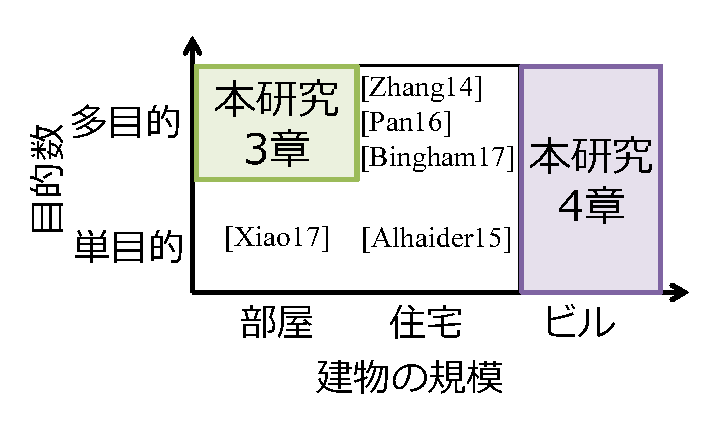
\includegraphics[width=0.6\textwidth,keepaspectratio=true]{fig/intro_position_objective.eps}
    \end{center}
    \caption{本研究の3章および4章の位置付け}
    \label{fig::intro_position_objective}
\end{figure}

\begin{figure}[ht]
    \begin{center}
        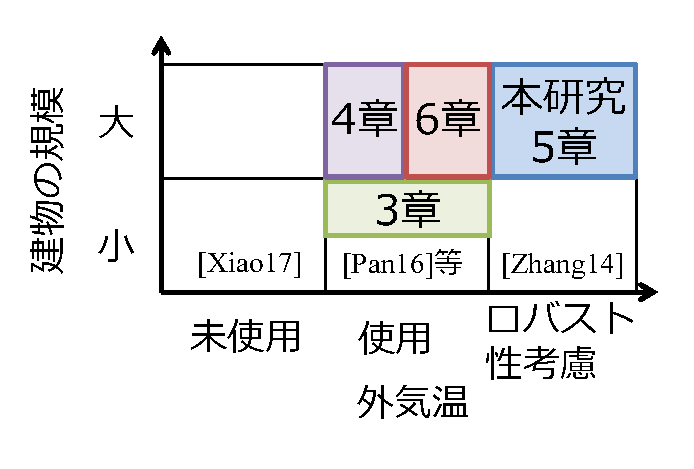
\includegraphics[width=0.6\textwidth,keepaspectratio=true]{fig/intro_position_robust.eps}
    \end{center}
    \caption{本研究5章の位置付け}
    \label{fig::intro_position_robust}
\end{figure}

\begin{figure}[ht]
    \begin{center}
        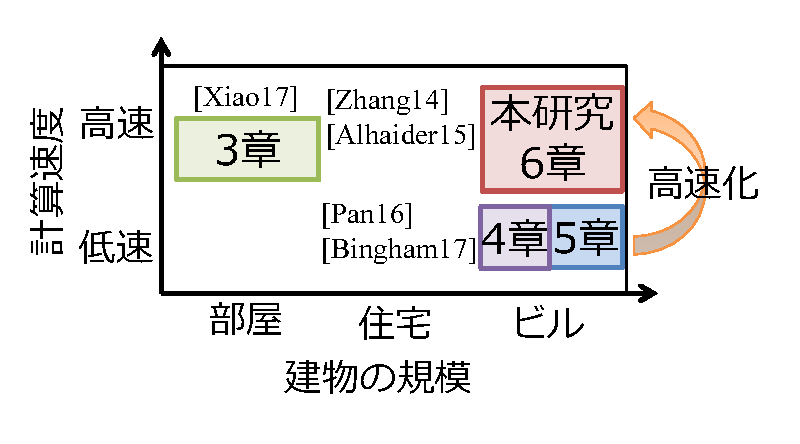
\includegraphics[width=0.6\textwidth,keepaspectratio=true]{fig/intro_position_speed.eps}
    \end{center}
    \caption{本研究6章の位置付け}
    \label{fig::intro_position_speed}
\end{figure}

\section{研究の位置付け}
上述の従来法と本研究におけるアプローチを,まず対象とするビル規模と目的数で分類したものを\figref{fig::intro_position_objective}に示す.目的関数の数を単目的とすると,上述のように重みや制約値の決定が難しく,また調整が困難であり,現場適用に課題がある.一方で目的関数の数を多目的とすると,どの程度快適度を犠牲にすることでエネルギー消費量を良い値にできるといったトレードオフ関係を考慮しつつ,適切なスケジュールを選択することができる.そのため,単一目的最適化で生じていた重みや制約値の調整の問題を解決できる.また,運用に変更があった場合にもエネルギー消費量や快適度の異なる他のスケジュールを適用することが容易であり,実利用に対して適した方法といえる.一方,対象ビル規模は,適用先によってさまざまであるが,一般に規模が大きくなるにつれ,大規模な熱源設備や空調設備が必要とされ,制御対象の面積・部屋数が増加するため,エネルギー消費量や快適度の予測および最適化が困難になる傾向にある.本研究では,中~大規模オフィスビルの空調設定スケジュールの最適化を対象とする.このようなビルでは,場合によってビルの部屋およびテナント単位の最適化も必要とされることから,まずオフィスビルの1部屋を対象として空調設定スケジュールの多目的最適化を行うコンセプトを提示する.その後,オフィスビル全体の多目的・単目的の空調設定スケジュール最適化の手法および結果について議論する.
次に,対象ビル規模と外気温の取り扱いで分類したものを\figref{fig::intro_position_robust}に示す.通常,ビルのエネルギー消費量および室内快適度には外気温が大きな影響を与える.計算を単純化するため,外気温を考慮しない数理モデルで最適化を行うアプローチが従来法にある\cite{Xiao17}.しかし,モデルによる目的関数算出を正確に行うためには外気温を考慮して目的関数計算する手法の採用が必要である.さらに実際には外気温が予報値に対して誤差を持つことから,これを考慮することでより実用性の高いスケジュールを獲得するアプローチがある.従来法\cite{Zhang14}ではモンテカルロ法により生成した複数の外気温予報シナリオの結果の発生確率による加重平均値を評価値として最適化するアプローチをとっていた.しかしながら,この手法では,1つの解を評価するためにシナリオ数の分の目的関数計算が必要であること,平均値を評価値とするため獲得できるスケジュールは予報値で最適化した結果に近い値に収束すること,ロバスト性を考慮せず目的関数値を良くした解は同時には得られないこと,などの問題があった.本研究では,実際の気象予報誤差データから上方・下方予報誤差のうち$\pm 2\sigma$の誤差分布までを考慮し,ロバスト性も目的とした多目的最適化アプローチによる空調設定スケジュールの最適化を5章にて実施している.これらのようなアプローチをオフィスビルに対して適用した例はこれまでにない.既設ビルのうち多くを占めるオフィスビルにおいて,この手法が有効であることを検証する.
さらに,対象ビル規模と計算速度について分類したものを\figref{fig::intro_position_speed}に示す.通常,対象ビル規模が大きくなるほど,快適性およびエネルギー消費量を算出するために計算しなければならない空調設備モデルや室モデルの数が増加するため,計算速度も低下する傾向にある.さらに,部屋や住宅の単位であればその計算モデルは数理モデルで記述が容易な規模であるが,規模の大きなビルになるとその計算モデルを逐一記述することは困難になってくる.そこで,ビルの構造や設備等の情報からモデルを定義し計算を行うシミュレータの利用が必須となる.シミュレータの内部構造は詳細な多数の数理モデルがビルモデルに合わせて結合されたものであることから,計算時間は多くかかることが一般的である.そこで,目的関数計算をサロゲートモデルで近似することが行われる.従来法\cite{Tresidder12}では,クリギング法を用いて設計変数ベクトルから目的関数値を直接近似するサロゲートモデルを用いる方法が考案されている.しかしながら,クリギング法では変数の数が多い場合に近似性能が悪化してしまうこと,近似対象の関数が連続値であることを想定した手法であるため,制約違反量のような非線形関数の近似は困難であることが問題であった.本研究では,シミュレータの出力する時系列データをNNを用いて近似し,時系列データを用いて目的関数計算する手法を6章にて提案する.本手法によって多変数データの近似が可能となるだけでなく,得られた時系列データから目的関数・制約違反量を計算することで非線形な関数値も推測可能である.

\begin{figure}[ht]
    \begin{center}
        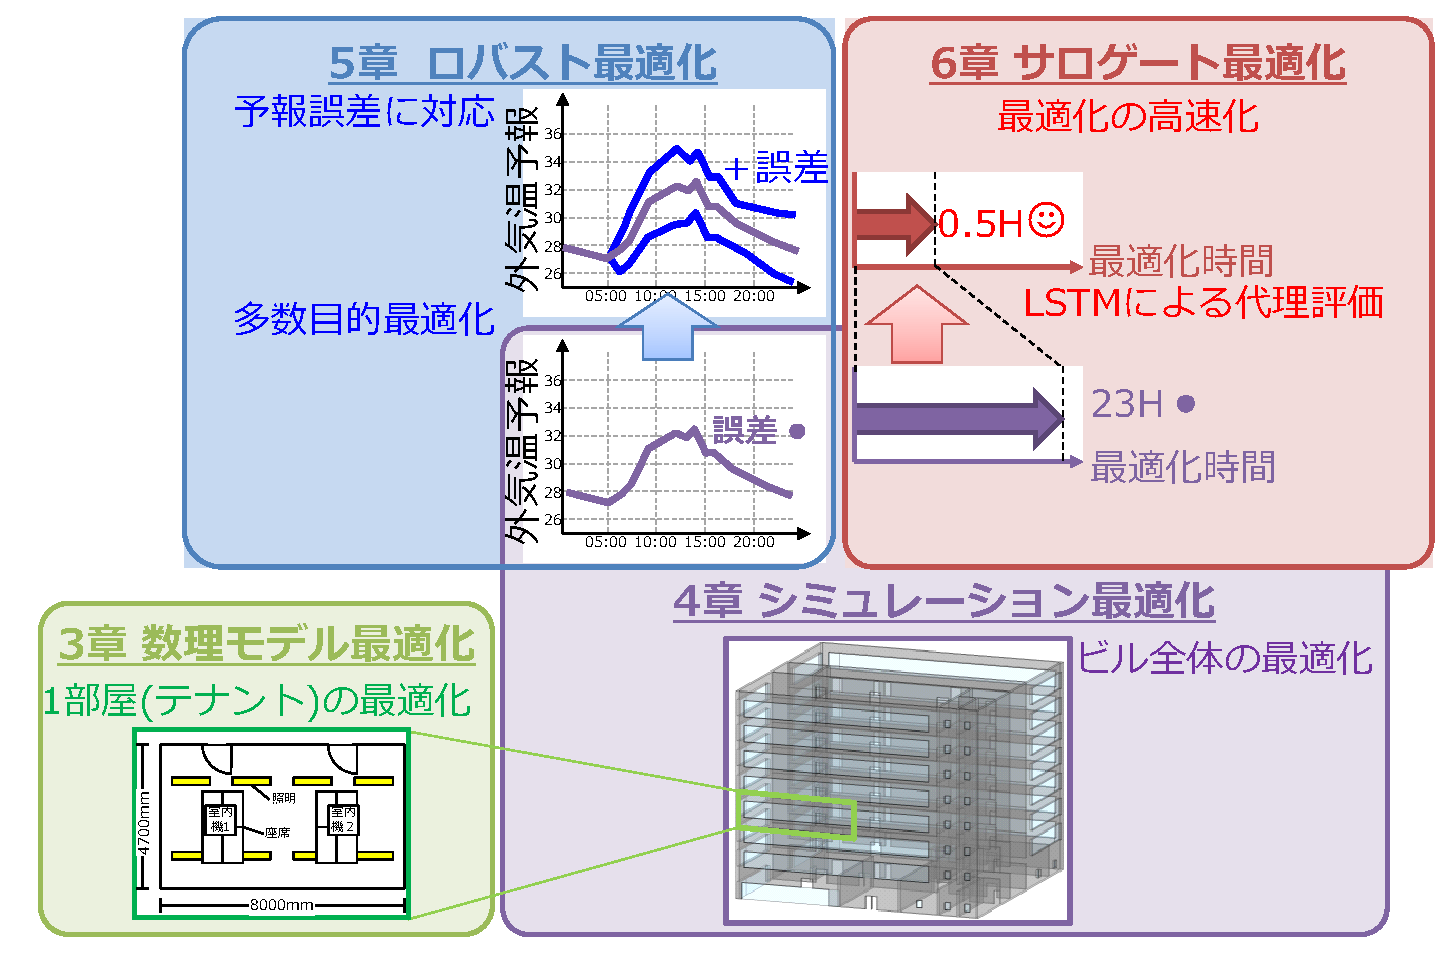
\includegraphics[width=1.0\textwidth,keepaspectratio=true]{fig/intro_bigpicture.eps}
    \end{center}
    \caption{本論文の全体像}
    \label{fig::intro_bigpicture}
\end{figure}

\section{本論文の構成}
%本論文の構成を以下に示す.
以下,2章では,本論文の展開に必要な進化計算に関する基礎的事項について述べ,3章以降に本論文で提案する方法について述べる.本研究で提案する方法の全体像を\figref{fig::intro_bigpicture}に示す.
2章では,多目的最適化問題と,その進化計算による解法について説明する.まず,多目的最適化問題とその解を求めるための基本的アプローチについて説明する.次に,多目的最適化の解探索手法として用いられる進化計算について,一般的な計算過程と解候補の生成方法,選択方法について説明する.その後,代表的な多目的最適化のための進化計算手法としてNSGA-IIおよびOMOPSOを取り上げ,そのアルゴリズムについて説明する.また,ほとんどの実問題が備える制約条件の考慮の方法について説明する.
3章では,オフィスビルの一部屋に対する空調設定スケジュール最適化問題を,従来行われてきた数理モデルにより定式化し,進化計算手法により最適化する手法を示す.空調設定スケジュール最適化問題の設計変数,目的関数,制約条件を定義し,これらの算出に必要な物理的要素,設備パラメータについて説明する.また,快適性の評価において重要な評価尺度であるPMVについて説明する.そして,この問題に対して進化計算を適用した場合に得られるパレート最適解集合とそのスケジュールの時系列データの分析を行う.
4章では,中規模ビルに対するシミュレーションモデルを構築し,シミュレーションモデルに基づいた評価を用いた進化計算手法により多目的最適化をする方法を示す.最適化対象とする中規模オフィスビルのフロアレイアウト,躯体・構造,壁・窓材料や各種設備について説明したのち,このビルを運用した場合のエネルギー消費量および快適度を算出するビルエネルギーシミュレーションモデルを構築する方法について詳細を述べる.また,このシミュレーションモデルによるシミュレーション結果から3章で述べた空調設定スケジュール最適化問題の目的関数,制約条件を計算する手順について説明する.その後,シミュレーションモデルによる評価に基づく多目的最適化によって獲得されたパレート最適解と,従来の設定温度を一定値として運用した結果との比較を行う.加えて,提案法の妥当性を検証するために,快適性の制約条件式を設けない場合との比較,快適性を目的ではなく制約とした場合の単一目的最適化結果との比較,他の多目的最適化手法による探索結果との比較,OMOPSOのアルゴリズム上の工夫の効果の比較を行う.
5章では,外気温の予報誤差に対してロバストな空調設定スケジュールを獲得する手法を示す.まず,気象庁が発表する外気温予報値と実績値を用いて実際の外気温予報精度を分析し,予報誤差を再現するシミュレーション用外気温データの設計手法を説明する.設計した予報誤差を含む外気温データを用いて,外気温予報誤差に対するロバスト性を示す2つの目的関数を定式化する.快適性・エネルギー消費量の2つの目的に加えて,ロバスト性を示す2つの目的関数を含む4目的の空調設定スケジュール最適化問題に対し,進化計算を用いてパレート最適解を探索する.獲得された外気温予報に対するロバストな空調設定スケジュールについて,従来の快適性・エネルギー消費量のみを考慮した場合の探索結果との比較を行う.さらに,4目的という多数目的最適化のクラスとなったロバスト空調設定スケジュール最適化問題に対して,複数の多目的・多数目的最適化手法による探索を試行し性能比較を行う.
6章では,シミュレータをサロゲートモデルにより簡素に代替することによる進化計算の総計算時間の短縮手法について提案する.4章で提案したシミュレーションモデルの入出力を,Recurrent Neural Network(RNN)の1つであるLSTMを用いて代替する手法の概要を説明する.また,LSTMによるサロゲート評価器の入出力,ネットワーク構成および学習手法を説明する.シミュレータの入出力データを学習データとして訓練したサロゲート評価器の予測精度について分析する.また,このサロゲート評価器を用いて多目的最適化した結果得られたパレート最適解について,サロゲート評価器とシミュレータそれぞれの出力結果を比較する.さらに,サロゲート評価器を用いた場合の最適化計算時間についてシミュレータとの比較を行い,サロゲート評価器による高速化の効果について分析する.加えて,同様の評価回数でもより良好な解を探索する,進化計算アルゴリズムの改良手法DOMOPSOを考案し,サロゲート評価器による多目的最適化問題に対して適用した結果について考察を行う.
最後に7章で本論文をまとめ,今後残された課題について述べる.
